\section{Case study}
% \yh{We may 1) change terms like the epoch 5, 40 to the $5^{th}$, $40^{th}$ epoch; and 2) Capitalize the first letter of each word in view names such as cluster view to the Cluster View.}

In this section, we demonstrate the effectiveness of MultiRNNExplorer in analyzing model behaviors and feature importance. 
We use the air pollutant data between 2015 to 2017 to train the model and use 8,375 cases in 2018 as testing data for analysis. 
% Notice that feature importance and hidden unit response are calculated on testing data,  
% The testing dataset contains the 8,375 individual cases in the year 2018.
\QM{The models training are conducted on a workstation with 2 $\times$ Intel Xeon E5-2650 v4 CPUs and 4 $\times$ Nvidia Titan x (Pascal Architecture) 12GB GDDR5X graphics cards.}
The hyper-parameters, \QM{average training time (seconds)} and accuracy of different models are listed in Table~\ref{table:model_configuration}. 
We demonstrate our system to the domain expert and analyze the trained models on several tasks.

\begin{table}[h!]
\centering
\caption{Configuration and performance of RNNs, including vanilla RNN, GRU, LSTM, and the RNNs with dense layer (e.g., RNN-Dense). The performance is evaluated by the mean square error (MSE) of $PM_{2.5}$; low MSE represents better performance.\yh{need discussion}}
\begin{tabular}{p{1.8cm}|p{0.5cm}|p{1.7cm}|p{0.5cm}|p{1.7cm}} 
 \hline
 Model & Size & Dense Layer & Time & MSE ($PM_{2.5}$) \\ [0.5ex] 
 \hline
    Vanilla RNN&100&No&364&5.31 $\pm$ 0.98 \\
    GRU&100&No&1081&4.32 $\pm$ 0.51\\
    LSTM&100&No&1377&4.81 $\pm$ 0.31\\
    GRU-Dense&100&3&1387&4.25 $\pm$ 0.21\\
    LSTM-Dense&100&3&1525&4.53 $\pm$ 0.53\\
\hline
\end{tabular}
\label{table:model_configuration}
\end{table}


\subsection{Changes Over Epochs}
To explore the model behavior over the training process, we manually select the RNN model trained after 5, 40, 120, and 200 epochs. Fig.~\ref{fig:evolution_epochs} shows the projections and top five most important features at different epochs.

In the Projection View (Fig.~\ref{fig:evolution_epochs}A), we choose $PM_{2.5}$ as the target feature and use a sequential color schema to indicate the predicted value where a darker color indicates a higher $PM_{2.5}$. 
At early stages ($5^{th}$ and $40^{th}$ epochs), we find that the points in a darker color are distributed uniformly in the projection and are mixed together with the points with a light color. 
This indicates that the cluster gradients are not able to present the distribution of the target feature yet.
After training more epochs, the dark points become more concentrated. 

In addition, the Feature Importance View (Fig.~\ref{fig:evolution_epochs}B) shows that the magnitude of the gradient starts from a small value and then keeps increasing in the training process. 
We also find that in the $5^{th}$ and $40^{th}$ epochs, the top five important features are $\color{PM25Color}{PM_{2.5}}$ and $\color{PM10Color}{PM_{10}}$ while in the $120^{th}$ epoch, the feature of wind speed is also ranked in the top five most important features. 
In the $200^{th}$ epoch, more features related to wind speed are listed in the top five features.
Another finding is that in the $5^{th}$ epoch, we observe that only the features from the last time steps are considered important while the models at the $40^{th}$, $120^{th}$, and $200^{th}$ epochs leverage more timestamps in the forecast.  
The domain experts indicate that the $PM_{2.5}$ and $PM_{10}$ at nearby locations are the most intuitive features to forecast $PM_{2.5}$ ($PM_{10}$ and $PM_{2.5}$ are always highly correlated).
Moreover, the last time step is very important because it is the closest one to the final prediction. 
Based on these observations, we infer that the features that are directly related with the targeted air pollutant are considered important in the early stage of the training process.
After more epochs, the model starts to learn other features that may indirectly influence the forecast, such as the \textit{\color{WINDColor}{Wind Speed}} and other pollutants ($\color{SO2Color}{SO_2}$ or $\color{NO2Color}{NO_2}$) (shown as Fig.~\ref{fig:evolution_epochs}B, 20$^{th}$,200$^{th}$ epochs). 

\UC{According to official website of United States Environmental Protection Agency (EPA): ``$SO_x$ can react with other compounds in the atmosphere to form small particles. These particles contribute to particulate matter (PM) pollution"\cite{SO2TOPM25}.
We also discussed the reason that $SO_2$ becomes important later in training with the domain experts. 
They said it is also possible that the $SO_2$ relates some industrial activity which results in the high-air pollutant. }
% They explained that the sulfur oxides ($SO_x$) react with other compounds in the air and form tiny particles which contribute to the particulate matter. 
% A "Report on the Environment" from the EPA (United States Environmental Protection Agency) indicates that ``SO2 emissions are an important environmental issue because they are a major precursor to ambient $PM_{2.5}$ concentrations"\cite{SO2TOPM25}.
Moreover, the domain experts explain that the wind speed is important for several reasons: 1) the air pollutants will  be blown away if the wind speed is high; 2) since the north and west of the target location have more factories which are the major source of air pollutants, the appropriate wind speed and direction will bring the air pollutants to Hong Kong.
Moreover, the data also show different patterns in the Cluster View during the training process. 
For example, as shown in \QM{Fig.~\ref{fig:evolution_epochs}C}, we found that in the $5^{th}$ epoch almost all three types of features: \textit{\color{SLPColor}{Sealevel Pressure}}, \textit{\color{DPColor}{Dew-point}} and  \textit{\color{SPColor}{Station Pressure}} are grouped into one cluster. 
After the $40^{th}$ epoch, we notice that this cluster is split into two clusters.
With these observations, we derive the conclusion that the model gradually learns the high-level knowledge in the training process.

\begin{figure}[t]
	\centering
	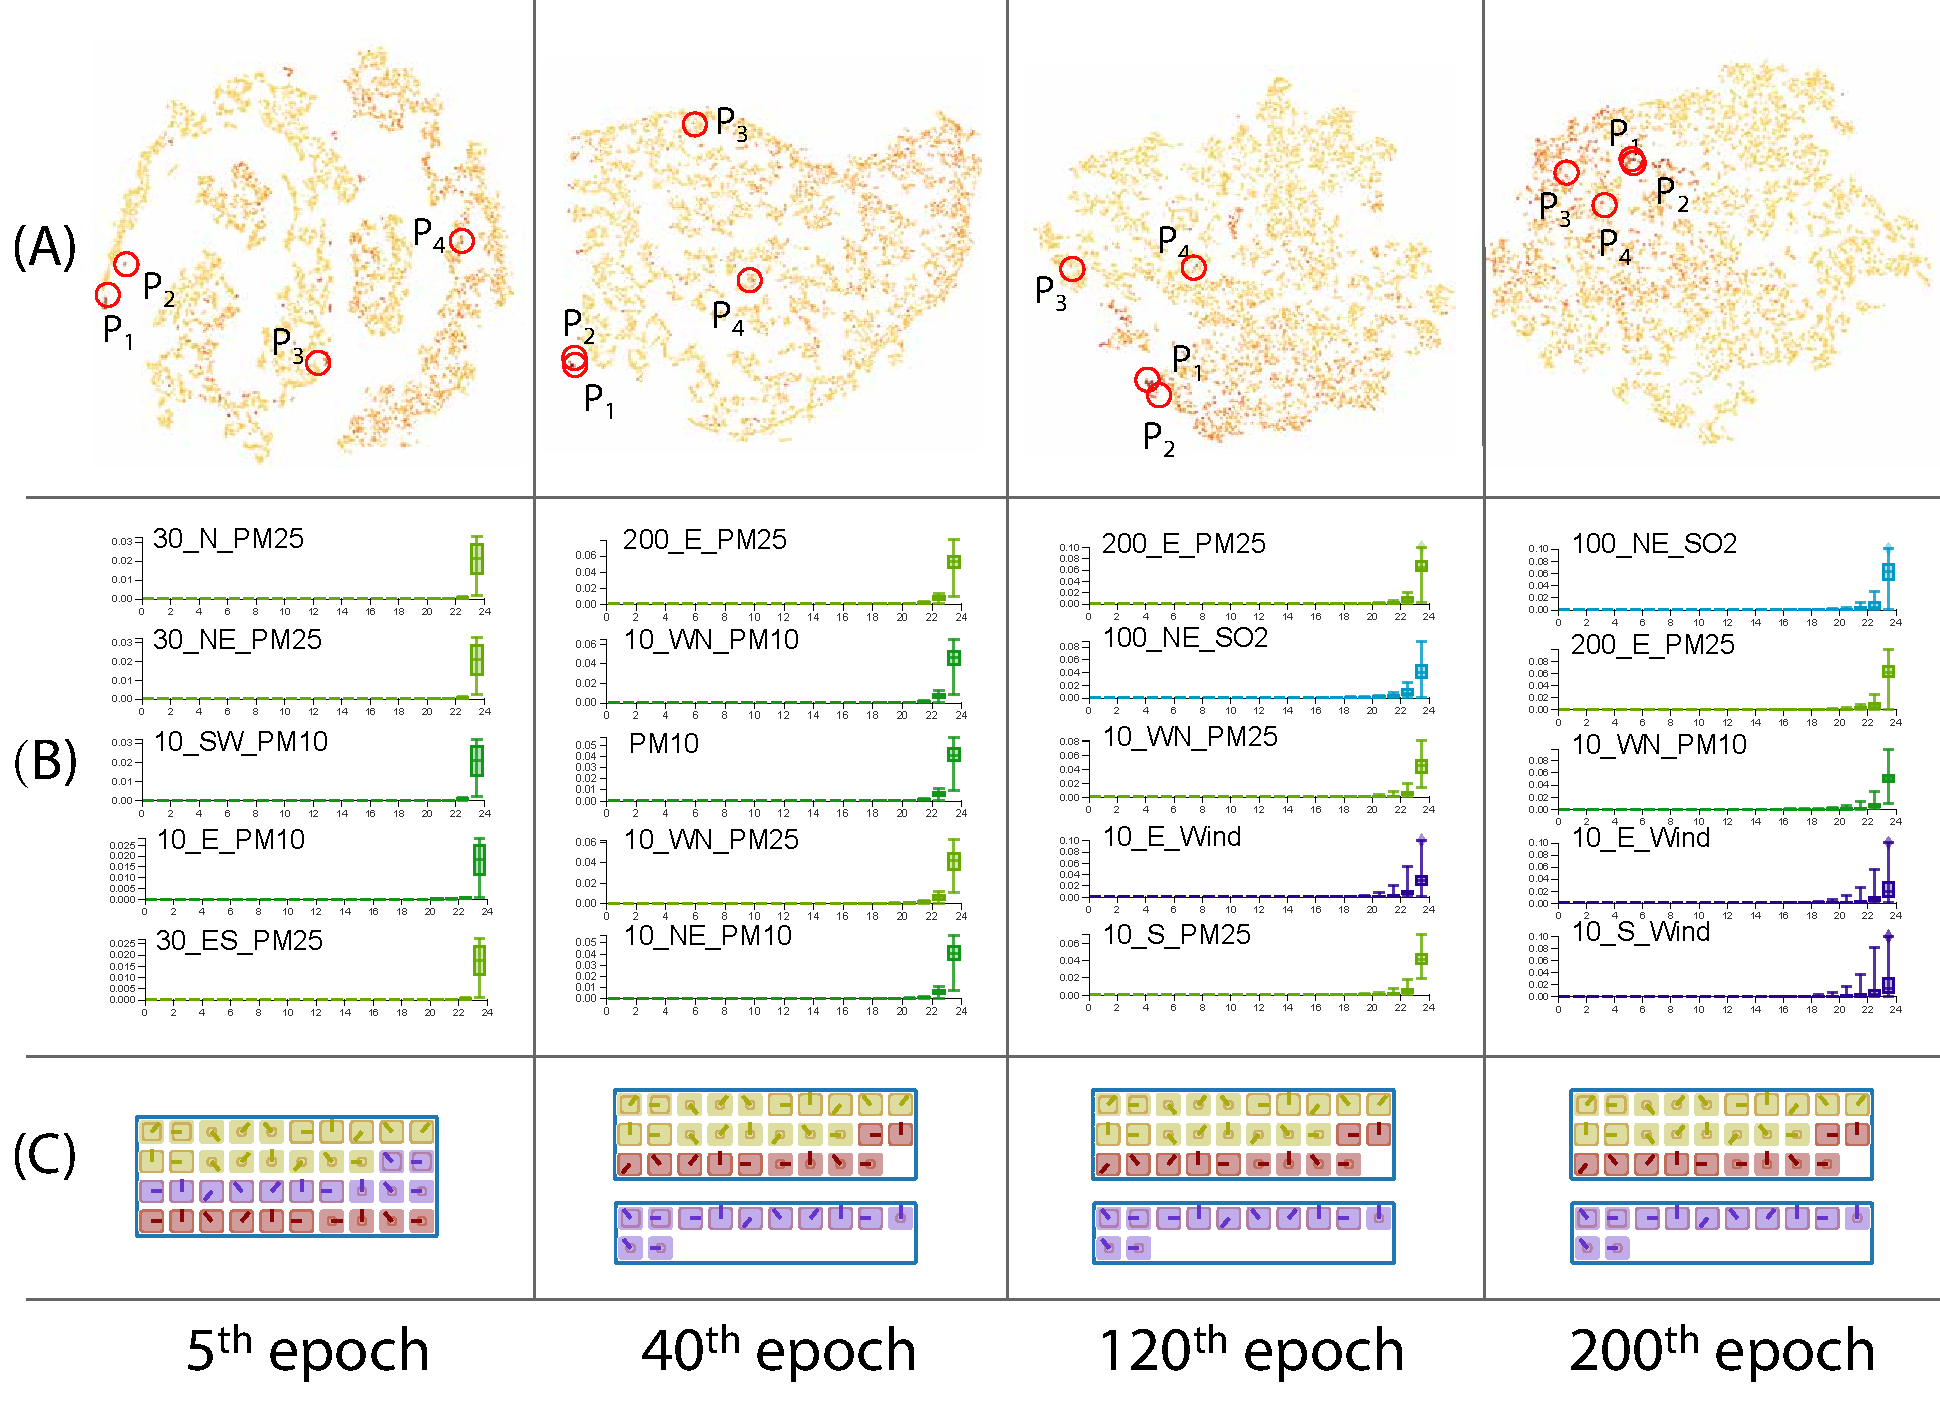
\includegraphics[width=0.45\textwidth]{pictures/Evaluation/evolution_epochs.pdf}
	\vspace{-3mm}
	\caption{\UC{The RNN model shows different behaviors along the training process. A, B, and C show the Projection View, top five important features, and feature clusters respectively at different epochs.}
% 	A: Projection Views shows the high-pollutant points gradually gathered during the training process; B: the top five important features at the corresponding epochs; C: the feature cluster change at each epoch.
	}
	\label{fig:evolution_epochs}
	\vspace{-4mm}
\end{figure}



\subsection{Understand Model Behaviors}
\begin{figure}[t]
	\centering
	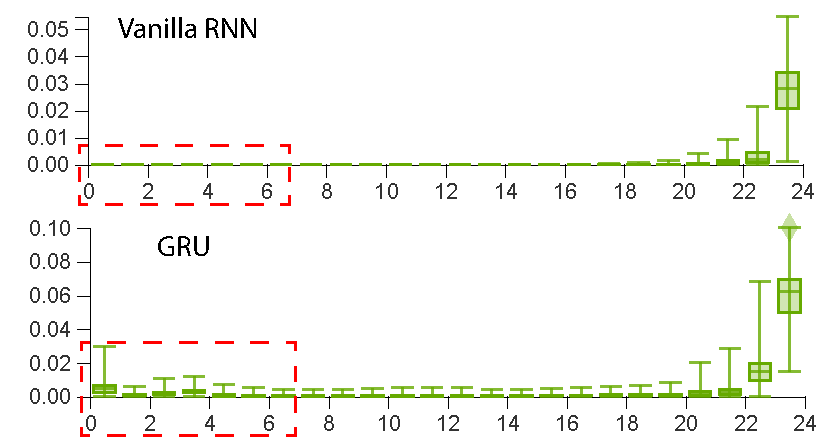
\includegraphics[width=0.40\textwidth]{pictures/Evaluation/FI_comparison.pdf}
	\vspace{-3mm}
	\caption{Compare the temporal importance of \textit{100\_NE\_PM25}  across different models. The dashed rectangle show both GRU has a "tail" while vanilla RNN does not.}
	\label{fig:gru_vs_rnn}
	\vspace{-4mm}
\end{figure}

\subsubsection{Model Mechanism}
This case study is conducted to understand what RNN models learn and to compare different models trained for air pollutant forecasting. 
With RNNExplorer, we are able to select models at any epoch. Fig.\ref{fig:teaser}A shows the Cluster View of GRU-Dense; by observing the cluster of features, we find that the features with same feature types are likely to cluster together such as the \textit{\color{RHColor}{Relative Humidity}} and \textit{\color{DPColor}{Dew-point}}, are exactly grouped into two separated clusters shown as Fig.~\ref{fig:teaser}A$_4$.
Moreover, we find that the $\color{PM25Color}{PM_{2.5}}$ and $\color{PM10Color}{PM_{10}}$ are always clustered together as shown in Fig. \ref{fig:teaser}A$_1$ and Fig. \ref{fig:teaser}A$_2$.
The domain expert explains that $\color{PM25Color}{PM_{2.5}}$ and $\color{PM10Color}{PM_{10}}$ are highly correlated because they are always generated together.
% On the other hand, we notice that all the features on \color{PM25Color}{$PM_{2.5}$} and \color{PM10Color}{$PM_{10}$} are also grouped by the distance: Fig. \ref{fig:teaser}A$_1$ and A$_2$ show that the features far away from (200km and 300km) or nearby (closer than 30km) the target location are clustered in different groups. 
This  shows that the model GRU-Dense is able to learn the information related to spatial locations.  

% Another thing of interest is the hyper-parameters of the model such as the RNN size. 
% \yh{How the hidden unit size relates with the observation below?}
% In the cluster view, we notice that a cluster of hidden units have very weak relationship to feature clustersi(Fig. \ref{fig:teaser} a4. \QM{explain?}.
% Such pattern also appears in the exploration of other models.

\begin{figure}[t]
	\centering
	\includegraphics[width=0.45\textwidth]{pictures/Evaluation/seasonal_behavior.pdf}
	\vspace{-3mm}
	\caption{Projection View across four seasons whose time range are defined by local standards.}
	\label{fig:seasonal_feature}
	\vspace{-4mm}
\end{figure}

\subsubsection{Feature importance}
We select the individual sequences of Fig.\ref{fig:teaser}D$_2$ and re-sort the features by the importance. 
From the Feature Importance View, the top important features are listed as Fig.\ref{fig:teaser}C, and we observe that most of them are related to feature $\color{SO2Color}{SO_{2}}$ and \textit{\color{WINDColor}{Wind Speed}}.
Then, top features change to $\color{SO2Color}{SO_2}$ and $\color{PM25Color}{PM_{2.5}}$ in later epochs. 
This observation shows that feature importance may vary across different individual cases. 
By default without selecting any sequences, the features are ranked according to their average importance over of all the test cases. 
We find that the \textit{\color{WINDColor}{Wind Speed}} is a major factor that influences the forecast because the wind related features are ranked in front.
% ~\yh{how? larger wind speed indicates higher predicted value?}. 
The domain experts point out that as there are very few factories in Hong Kong, the local emissions are not a major reason that influences the forecast result. 
Instead, the $PM$ pollutants are easily transported from the north, west, and east of mainland China, thus the $wind$ plays an important role in the forecast of $\color{PM25Color}{PM_{2.5}}$ and $\color{PM10Color}{PM_{10}}$.
% 0.76
% \begin{figure*}[ht]
% 	\centering
% 	\includegraphics[width=1\textwidth]{pictures/Evaluation/winter_exploration.pdf}
% 	\vspace{-3mm}
% 	\caption{
% 	Case exploration for the $PM_{2.5}$ forecast in winter. A, B) Filter and highlight the individual cases in January 2018; C1, C2) Two groups of individual cases are selected by brushing; D) The top 10 importance features for the group selected in C1; E1, E2) Representative cases of C1 and C2.}
% 	\label{fig:winter_exploration}
% 	\vspace{-4mm}
% \end{figure*}

\begin{figure}[t]
	\centering
	\includegraphics[width=0.45\textwidth]{pictures/Evaluation/winter_exploration.pdf}
	\vspace{-3mm}
	\caption{	Case exploration for the $PM_{2.5}$ forecast in winter. A, B) Filter and highlight the individual cases in January 2018; C1, C2) Two groups of individual cases are selected by brushing; D) The top 10 importance features for the group selected in C1; E1, E2) Representative cases of C1 and C2.}
	\label{fig:winter_exploration}
	\vspace{-4mm}
\end{figure}
During the exploration of different models, we notice that the temporal pattern of the Feature Importance View is very different across different models. 
Fig.\ref{fig:gru_vs_rnn} compares the feature importance for vanilla RNN and GRU.
With the selected feature of \textit{100\_NE\_PM25}, one observation is that the Feature Importance Views of model GRU has a ``tail" (Fig.\ref{fig:gru_vs_rnn}) especially for the first three timestamps, while we do not observe similar patterns in vanilla RNN.
% While the corresponding feature for vallina RNN have no such kind of pattern. 
This solves one question raised by the domain experts: is it necessary to use such complex models like RNN to conduct air pollutant forecasting tasks?
It is a controversial question~\cite{brownlee2017long} as in some applications all important information is included within within recent small time ranges~\cite{gers2002applying} and do not necessarily require complex machine learning models. 
However, by using our system, we can find that the GRUs are able to memorize more long-term information than vallina RNNs. 
Since the air pollutant and meteorology features (such as temperature) have a daily periodic pattern, the input features around 24 hours ahead are also considered relevant to the forecast. 
In addition, we can observe that the GRU models have better performance compared with vanilla RNNs from Table~\ref{table:model_configuration}. 
% ~\yh{requires some logic to connect to gated RNN.}
We think the gate RNNs are applicable for the air pollutant forecast. 



\subsection{Case exploration}

In Hong Kong, air quality always shows seasonal patterns such as the ``large winter-summer contrasts in $PM_{2.5}$ mass" due to the Asiatic monsoon~\cite{louie2005seasonal}. We conduct this case study to understand the model behavior in different seasons.  

\subsubsection{Overview of the model behavior across seasons}

The Projection View allows users to select individual cases according to different times by brushing on the timeline (Fig.~\ref{fig:teaser}E) and provides an overview of all cases (\textbf{T5}).
We first choose the GRU-Dense model and target feature of $PM_{2.5}$.
We gradually select the time ranges to roughly filter the cases in winter, spring, summer, and fall. 
The unfiltered sequences are colored in light grey to highlight the selected cases as shown in  Fig.~\ref{fig:seasonal_feature}. 
We found that the fall and winter sequences are clustered at the left-bottom part of the whole figure (Fig.~\ref{fig:seasonal_feature}A,D). 
The sequences in summer gather at the right-top part (Fig. \ref{fig:seasonal_feature}C), while the sequences in spring are distributed in different locations compared with the other three seasons (Fig.\ref{fig:seasonal_feature}B).
Even though some outliers exist in the Projection View as shown in Fig.~\ref{fig:seasonal_feature}A$_1$,C$_1$, we can find the model can capture the complex seasonal features in data. 

\subsubsection{Explore the model behavior in winter}

Furthermore, we notice that several sequences indicate the target location has a serious $PM_{2.5}$ pollutant in winter. 
In the Projection View, we first select the time range of January 2018 (Fig.~\ref{fig:winter_exploration}A) to highlight all the cases in this time range (Fig. \ref{fig:winter_exploration}B). 
We notice there are many cases are colored in dark red, which indicates these cases suffer a heavy $PM_{2.5}$ pollutant (Fig.~\ref{fig:winter_exploration}C1).
We select these sequences to explore their feature importance distributions and rankings.
The top ten important features are \textit{\color{WINDColor}{Wind Speed}}, $\color{PM25Color}{PM_{2.5}}$ and $\color{PM10Color}{PM_{10}}$.
The selected sequences also appear in the Individual Views; all these sequences form one stack, and we choose one of them as an example as shown in Fig.~\ref{fig:winter_exploration}E$_1$. 
In the Cluster Importance Chart, cluster 3, 6, and 7 show great influence in the forecast. 
These corresponding feature clusters are shown in Fig.~\ref{fig:winter_exploration}E$_3$, which presents the clusters of $PM_x$ and \textit{Wind Speed} respectively. 
The above exploration further indicates that the most important features in the forecasting are about $\color{PM25Color}{PM_{2.5}}$, $\color{PM10Color}{PM_{10}}$, and \textit{\color{WINDColor}{Wind Speed}}. 

The domain expert states: ``During winter, strong radiative cooling over the continent creates a high-pressure anticyclone that drives cold, dry polar air from the continent into the surrounding oceanic areas, resulting in weak to moderate northeasterly winds or strong northerly winds" \cite{louie2005seasonal, murakami1979winter}. 
The weak to moderate wind is able to bring the air pollutant from Pearl River Delta region in China, which is a highly populated region and has a lot of heavy industry \cite{cao2003characteristics}.
Thus, the major factors that mostly influence Hong Kong's air quality in winter are the air pollutants and the wind.
Specifically, the $PM_{2.5}$ and $PM_{10}$ from the north and east affects the prediction results the most. 

We are also interested in how different models behave between the high-pollutant and low-pollutant sequences in the winter. 
We select individual cases with low $PM_{2.5}$ from the Projection View as Fig.~\ref{fig:winter_exploration}C$_2$ shows, and two stacks if individual cases appear in the Individual View. 
By observing the representative case (Fig.\ref{fig:winter_exploration}E$_2$), we find a cluster which is very important at the last timestamp in the Cluster Importance Chart (Fig.~\ref{fig:winter_exploration}E$_4$), which indicates nearby $PM_{2.5}$ and $PM_{10}$. 
Both the Top Feature List (Fig.~\ref{fig:winter_exploration}E$_5$) and the Cluster Importance Chart show that the features of recent time steps are very important for the forecast, which is different from the heavy pollution sequences (Fig.~\ref{fig:winter_exploration}E$_6$). 
We guess that for the low air pollutant (target feature) cases, only recent important features are leveraged by the model. 










